\renewcommand{\encodingdefault}{OT1}
\documentclass[conference]{IEEEtran}
\IEEEoverridecommandlockouts
% The preceding line is only needed to identify funding in the first footnote. If that is unneeded, please comment it out.
\usepackage{cite}
\usepackage{amsmath,amssymb,amsfonts}
\usepackage{algorithmic}
\usepackage{graphicx}
\usepackage{textcomp}
\usepackage{xcolor}
\usepackage{hyperref}
\usepackage{minted}
\def\BibTeX{{\rm B\kern-.05em{\sc i\kern-.025em b}\kern-.08em
    T\kern-.1667em\lower.7ex\hbox{E}\kern-.125emX}}
\begin{document}

\title{Jitsi on OpenBSD\\
{\Large Puffy presents video conferencing}
}

\author{\IEEEauthorblockN{Philipp Buehler}
\IEEEauthorblockA{
\textit{sysfive.com GmbH}\\
Hamburg, Germany \\
pb-openbsd@sysfive.com}

}

\maketitle

\begin{abstract}
This paper will cover all bits and bolts to fully understand the components
at play, their intercommunications and how this knowledge can be used to create
a Jitsi-on-OpenBSD setup that features a restricted (compartmentalized) setup using
dedicated machines or -as shown- VMM based VMs, where each VM runs only one of the
components.

It'll be documented what's necessary to create a sensible pf.conf on each VM and how to
add reverse proxy (relayd, haproxy) for distribution of workload.

Also covering pitfalls/hints along underlying components and what to lookout for on 
the client/browser side for interopability.
\end{abstract}

\begin{IEEEkeywords}
Jitsi, OpenBSD, VMM
\end{IEEEkeywords}

% XXX
%\section{Examples}
%Just some template code
%\begin{minted}{c}
%int main(){
% printf("hello");
%}
%\end{minted}
%\subsection{Units}
%\begin{itemize}
%\item Use either SI (MKS) or CGS as primary units. (SI units are encouraged.) English units may be used as secondary units (in parentheses). An exception would be the use of English units as identifiers in trade, such as ``3.5-inch disk drive''.
%\item Use a zero before decimal points: ``0.25'', not ``.25''. Use ``cm\textsuperscript{3}'', not ``cc''.)
%\end{itemize}
% XXX

\section{Introduction}
Jitsi and OpenBSD are both not covered much as a documented setup. Installation documents
for Jitsi are almost always about Linux OS (and there mostly Debian) and do not cover
some internals. The reference documentation on the other hand can be very overwhelming.

There is some FreeBSD ``all in one'' port (package) with no explanation and it cannot be
used to install core components (only) on different nodes.

This documentation is to show a distributed install on OpenBSD using pre-packages and
need-to-function (minimum) firewall settings (`pf.conf`).

\section{Riddles}
Both major players show obstacles that have to be overcome to gain a functioning installation.
\subsection{Jitsi}
A "full blown" Jitsi installation can consist over over a dozen components and all the
necessary networking/firewalling configuration can be exhaustive. Any possible discovery
magic is not documented.

Some configuration snippets are undocumented and tend to make the understanding poorer
not better. Worst example are necessary DNS settings and `nginx.conf.`

The typical answer to be found on asking question is to use the official `all-in-one`
Debian VM.

\subsection{OpenBSD}
This also leds to the question if it's possible to run a (core) Jitsi installation on
OpenBSD only or if there's need be for Linux (VM).

Also it's a bit difficult to find example-based documentation on VMM, e.g. for using
VMM as the core router, too. (Combination `vm.conf`+`pf.conf`s).

Can we scale the installation horizontally and how to use Java based applications
with `rcctl`.
\section{Components}
\subsection{OpenBSD}
In this example setup I make heavy use of `VMM` eco system on OpenBSD which consists of:
\begin{itemize}
\item `vmm(4) - virtual machine monitor:`
    kernel driver isolating/providing the required resources for the VMs (“hypervisor”)
\item `vmd(8):`
	userland daemon to interact with `vmm`
\item `vmctl(8)`:
	administrative tool to create, start/stop, .. VMs
\item `vm.conf(5)`:
	persist VMs resource configuration
\end{itemize}
\subsection{Jitsi}
A `core` (basic video conferencing) setup comprised by:
\begin{itemize}
\item `nginx(8)` web:
	serving web assets and reverse proxy BOSH or websockets
\item `prosody(8)` xmpp:
	conference chat + internal components communication (esp. “PubSub” for health/discovery)
\item `jicofo` JItsi COnference FOcus:
	room+session handling in conferences (who’s talking to whom and where)
\item `jvb` videobridge:
	mediastream (WebRTC) handlings between participants (SFU)
\item `jibri` JItsi BRoadcasting Infrastructure (optional):
	recording + streaming conferences
\end{itemize}

\section{Architecture}
To host the Jitsi components in a VM each, this uses the following architecture (see Figure 1).
\begin{figure*}
    \centering
    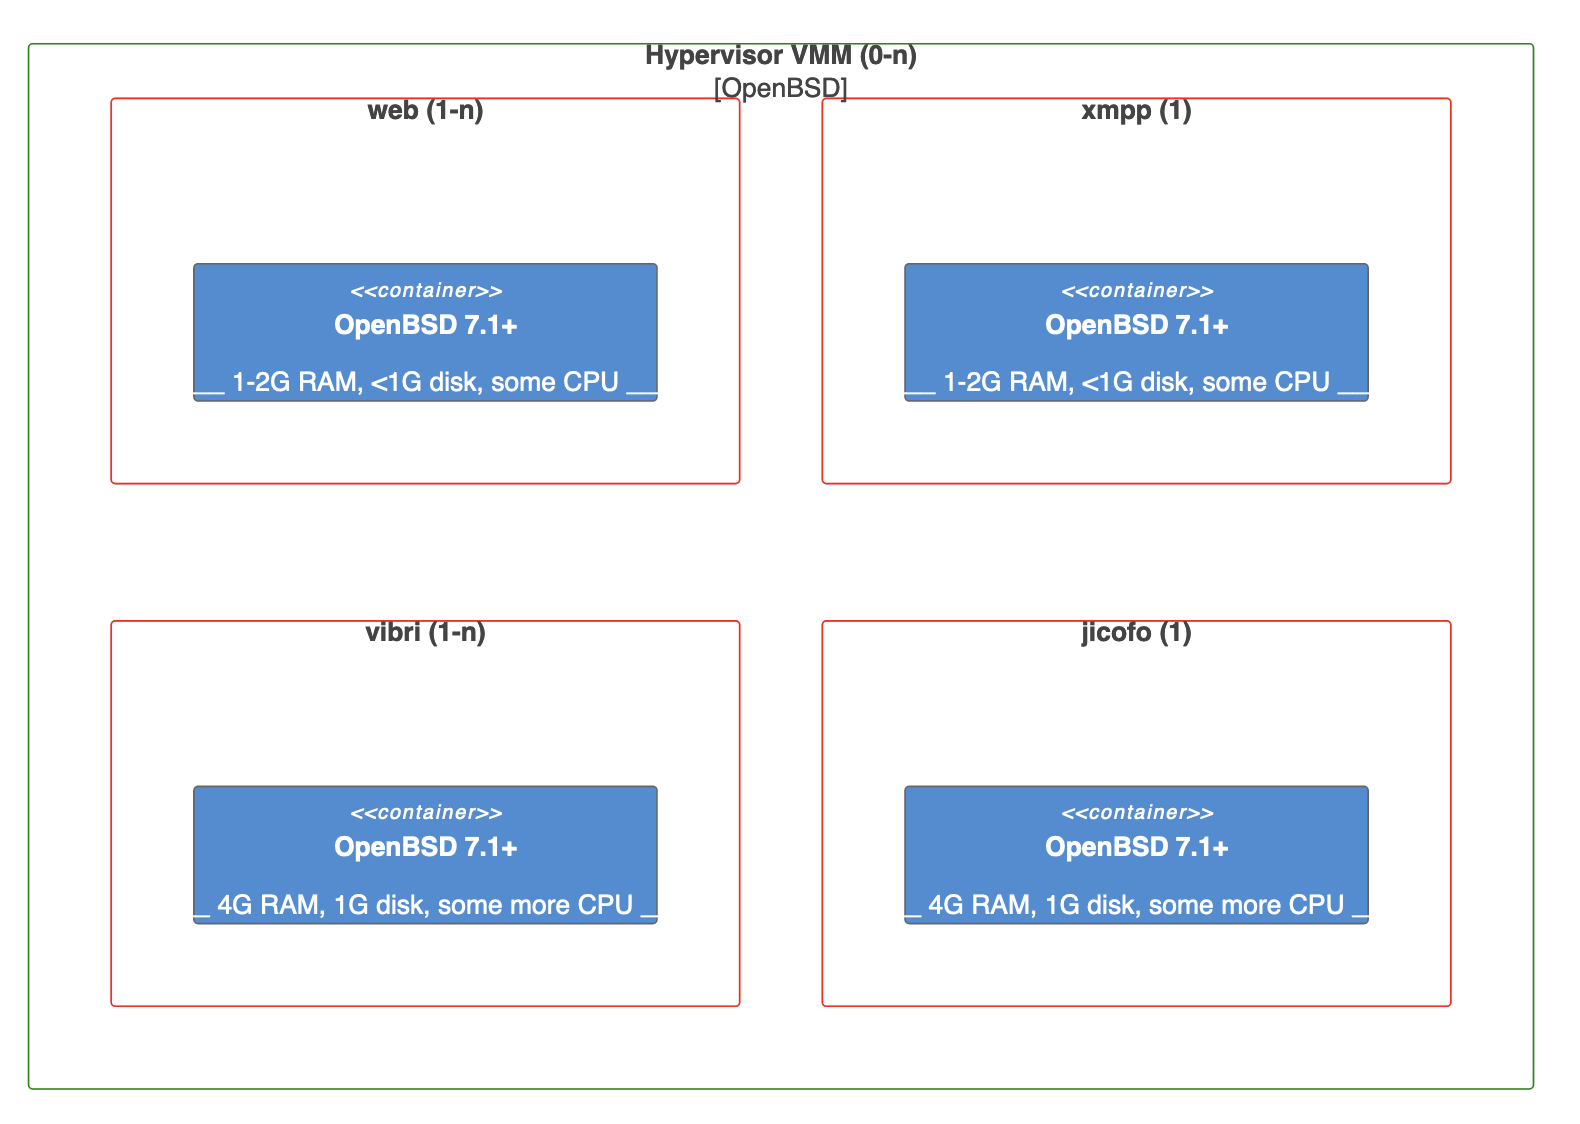
\includegraphics[width=18cm]{img/arch-openbsd.png}
    \caption{\textsf{OpenBSD VMM architecture}}
\end{figure*}
\section{Communications}
Communications between the components and the logical `publication` + `subscription` in Jitsi
is as follows (needed in `pf.conf` later on).
\begin{figure*}
    \centering
    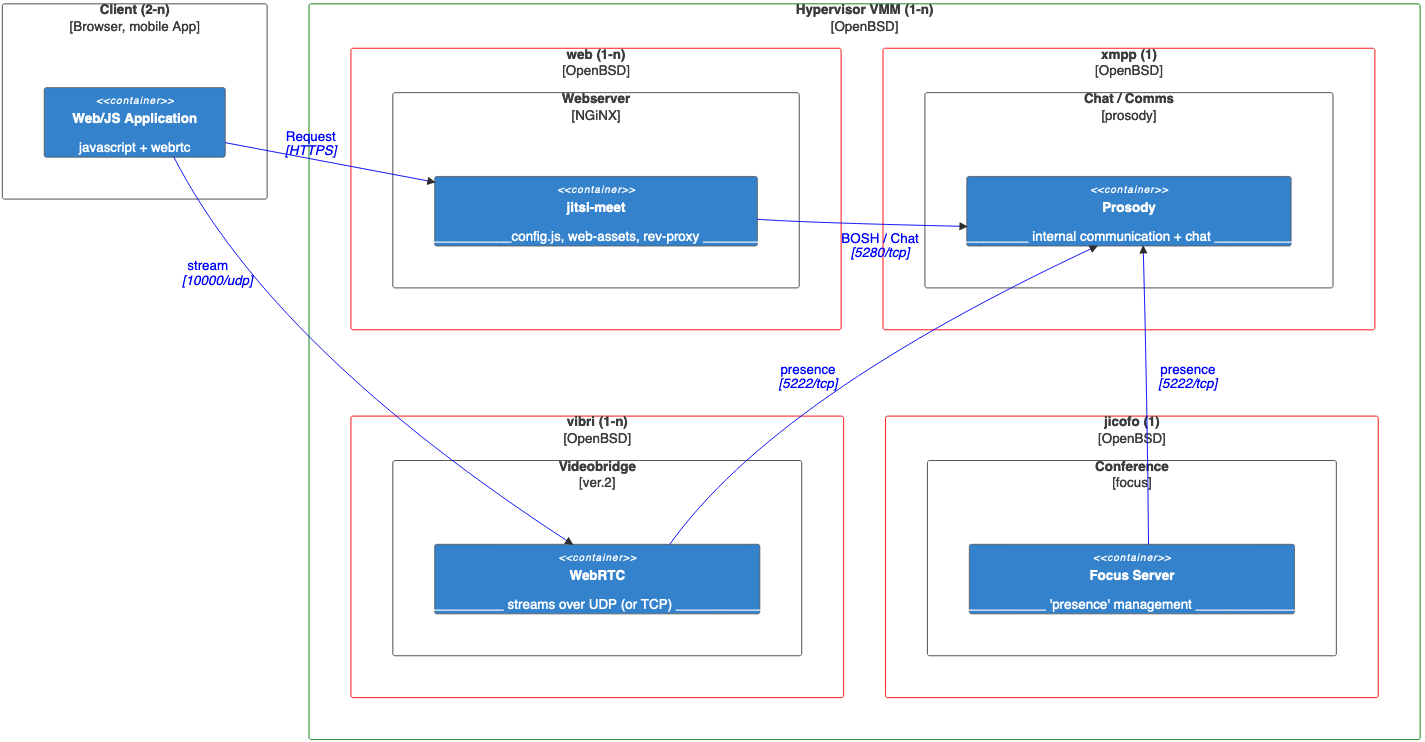
\includegraphics[width=18cm]{img/arch-tcp.png}
    \caption{\textsf{OpenBSD VMM architecture}}
\end{figure*}
\begin{figure*}
    \centering
    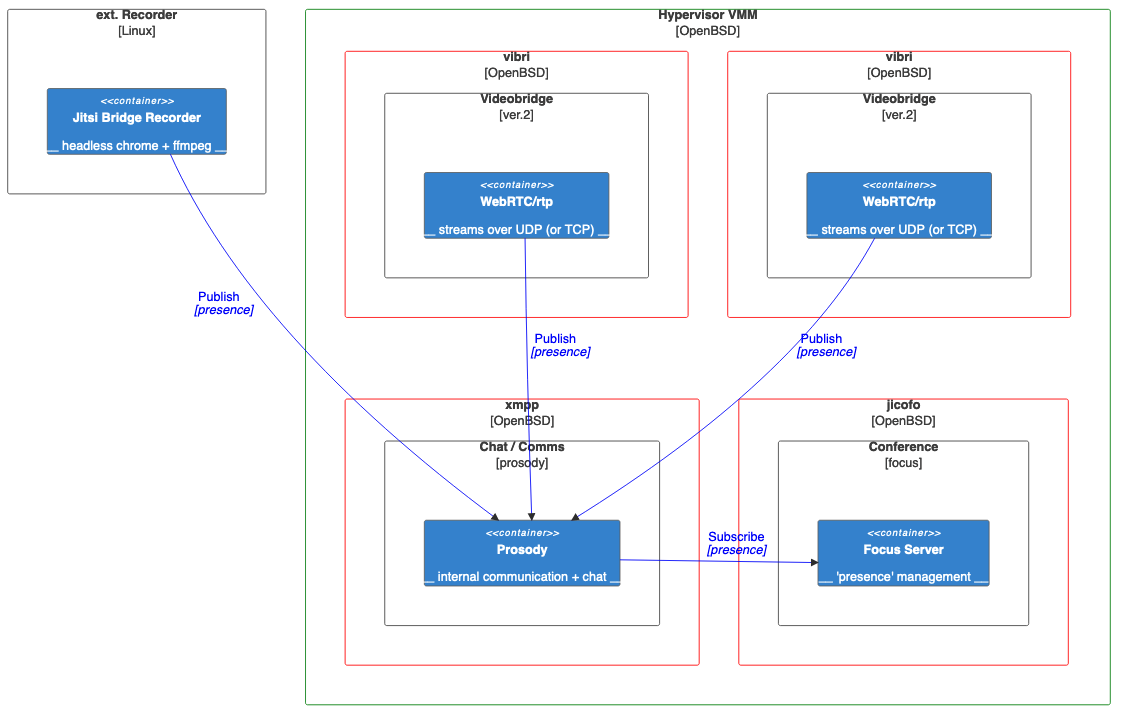
\includegraphics[width=18cm]{img/arch-pubsub.png}
    \caption{\textsf{OpenBSD VMM architecture}}
\end{figure*}

\section{Installation}
\section{Firewalling}
\subsection{VMM}
\subsection{web/nginx}
\subsection{prosody}
\subsection{jicofo}
\subsection{videobridge}
\section{Prosody}
\subsection{Users}
\subsection{TLS}
\section{nginx}
\subsection{web}
\subsection{misc}
\section{webclient}
\section{jicofo}
\subsection{Parameters}
\subsection{JVM}
\section{videobridge}
\subsection{Parameters}
\subsection{JVM}
\section{Pitfalls}
\subsection{OpenBSD}
\subsection{Jitsi}
\section{Status}
\section{Outlook}
\section{Acknowledgments}







\section{Availability}
This paper, presentation slides and other directly related resources can be found on github:
\url{https://github.com/double-p/presentations/AsiaBSDCon/2022/}


\begin{thebibliography}{00}
\bibitem{b1} OpenBSD project \url{https://www.openbsd.org/}
\bibitem{b2} Jitsi \url{https://github.com/jitsi/}

\end{thebibliography}

\end{document}
